% \begin{figure}[ht]
%     \centering
%     \includegraphics[width=0.575\columnwidth]{promasens/figures/methodology/kinematic_frames_v3_cropped.pdf}
%     \caption{Coordinate frames for a soft segment containing the $j^\mathrm{th}$ magnetic sensor and the $k^\mathrm{th}$ cylindrical magnet placed along the center line. $\{S_{i-1}\}$ and $\{S_{i}\}$ describe the frames of the base and tip of the $i^\mathrm{th}$ segment respectively.}\label{fig:promasens:kinematics_frames_soft_segment}
% \end{figure}

\section{Proprioception with magnetic sensors}

This section introduces a methodology to achieve proprioception for soft robots with magnetic sensors.
%
We consider a continuum robot with the shape of its backbone described by the configuration variables $q \in \mathbb{R}^{n_\mathrm{q}}$.
In the commonly used \gls{PCC} kinematic state parametrization~\cite{webster2010design}, the continuum robot is assumed to consist of $n_\mathrm{b}$ segments with each segment exhibiting constant curvature and elongation along its length. Therefore, the configuration of the soft robot can be described with $q \in \mathbb{R}^{3n_\mathrm{b}}$.
Please refer to Appendix~\ref{sub:promasens:kinematic_model_pcc} for more details.
We indeed use PCC for most of our simulations and experiments.
Note, however, that the proposed proprioception algorithm applies to any finite-dimensional kinematic description of a soft robot~\cite{armanini2023soft}.
Indeed, we also specifically consider a robot with affine curvature~\cite{della2020soft, stella2023piecewise} with its shape described by the configuration $q \in \mathbb{R}^4$. We document this alternative kinematic model in Appendix~\ref{sub:promasens:kinematic_model_ac}.
The proprioception methodology described in the remaining section is agnostic to the chosen kinematic model.
% For the sake of clarity, we use the \gls{PCC} kinematic state parametrization as proposed by \cite{della2020improved}. We consider a continuum robot described by $n_\mathrm{b}$ \gls{CC} segments and configuration variables $q \in \mathbb{R}^{3n_\mathrm{b}}$. Note, however, that the proposed method applies to any finite-dimensional kinematic description of a soft robot~\cite{armanini2023soft}.

\subsection{Proposed method at a glance}

%The shape of each segment can be parameterized with $q_i$.
We integrate $n_\mathrm{m}$ axially symmetric magnets and $n_\mathrm{s}$ magnetic sensors into the robot. The magnets must be installed along the center line of the segment while the sensors can be arbitrarily placed.
%
%To achieve proprioception of the entire robot shape, at least one magnet must be integrated into each segment.
%
Fig.~\ref{fig:promasens:methodology} concisely describes the proposed shape-sensing strategy with a pictorial example of a soft robot described with three constant curvature segments equipped with five magnetic sensors and three cylindrical magnets.
%

The goal of the algorithmic part (center of the figure) is to regress the robot shape (left) by estimating the configuration $\hat{q}$ of all segments (right),
%$q(t) \in \mathbb{R}^{3 n_\mathrm{b}}$
starting from the measurements of the magnetic sensors $u$ (e.g. usually the magnetic flux density).
We achieve this by training a sensor measurement predictor and subsequently optimizing the configuration estimate $\hat{q}$ for the prediction $\hat{u}$ to match the actual sensor measurement $u$.
Instead of predicting the sensor measurements end-to-end, we decouple the kinematics by explicitly describing the kinematic relationship $\hat{\xi}_j = f_{\xi,j}(\hat{q})$ between sensor $j$ and each magnet. % \hat{\xi}_j \in \mathbb{R}^{1+4 n_\mathrm{m}}
Then, we train a neural network $f_{\pi_j}$ to predict the measurement $\hat{u}_j$ based on the input $\hat{\xi}_j$.
To achieve proprioception, we jointly optimize $\hat{q}$ for all sensor measurement predictions. %We define a \gls{MSE} loss between the predicted and actual sensor measurements, and after back-propagating the loss, we perform gradient descent.

% PCC Kinematics with Elongation
% \subsection{Background: Piecewise Constant Curvature Kinematics}\label{sub:promasens:kinematic_model_pcc}

% The state of each segment $i$ of unextended length $L_{0,i}$ and radius $d_i$ is described by
% \begin{equation}
%     q_i = \begin{bmatrix}\Delta_{x,i} & \Delta_{y,i} & \delta L_i \end{bmatrix}^{\mathrm{T}} \in \mathbb{R}^3
% \end{equation}
% where $\Delta_{x,i}$ and $\Delta_{y,i}$ represent bending into the local x- and y-directions respectively and $\delta L_i$ defines the extension of the segment.
% The base frame of segment $i$ is referred to as $\{S_{i-1}\}$ as stated in Fig.~\ref{fig:promasens:kinematics_frames_soft_segment}. Given $q_i$, a homogeneous transformation $T_{i-1}^{i}(q_i)$ to the tip frame $\{S_{i}\}$ is available
% \begin{equation}
% \label{eq:promasens:transform_improved_q}
% \begin{split}
%     R_{i-1}^{i} &=
%     \begin{bmatrix}
%         1 + \frac{\Delta_{x,i}^2}{\Delta_{i}^2} \left ( \mathrm{c}_i - 1 \right ) & \frac{\Delta_{x,i} \Delta_{y,i}}{\Delta_{i}^2} \left ( \mathrm{c}_i - 1 \right ) & \frac{\Delta_{x,i}}{\Delta_i} \mathrm{s}_i\\
%         \frac{\Delta_{x,i} \Delta_{y,i}}{\Delta_{i}^2} \left ( \mathrm{c}_i - 1 \right ) & 1 + \frac{\Delta_{y,i}^2}{\Delta_{i}^2} \left ( \mathrm{c}_i - 1 \right ) & \frac{\Delta_{y,i}}{\Delta_i} \mathrm{s}_i\\
%         \frac{-\Delta_{x,i}}{\Delta_i} \mathrm{s}_i & \frac{-\Delta_{y,i}}{\Delta_i} \mathrm{s}_i & \mathrm{c}_i
%     \end{bmatrix},\\
%     t_{i-1}^{i} &= \frac{d_i ( L_{0,i}+\delta L_i)}{\Delta_i^2}
%     \begin{bmatrix}
%         \Delta_{x,i} (1 - \mathrm{c}_i) & \Delta_{y,i} (1 - \mathrm{c}_i) & \Delta_{i} \mathrm{s}_i,
%     \end{bmatrix}^{\mathrm{T}}
% \end{split}
% \end{equation}
% where we substituted $\Delta_i = \sqrt{\Delta_{x,i}^2 + \Delta_{y,i}^2}$, $\mathrm{s}_i = \sin \left ( \frac{\Delta_i}{d_i} \right )$, and $\mathrm{c}_i = \cos \left ( \frac{\Delta_i}{d_i} \right )$ for conciseness.

\begin{figure}[t]
\centering
\subfigure[Magnet Sensor Kinematics]{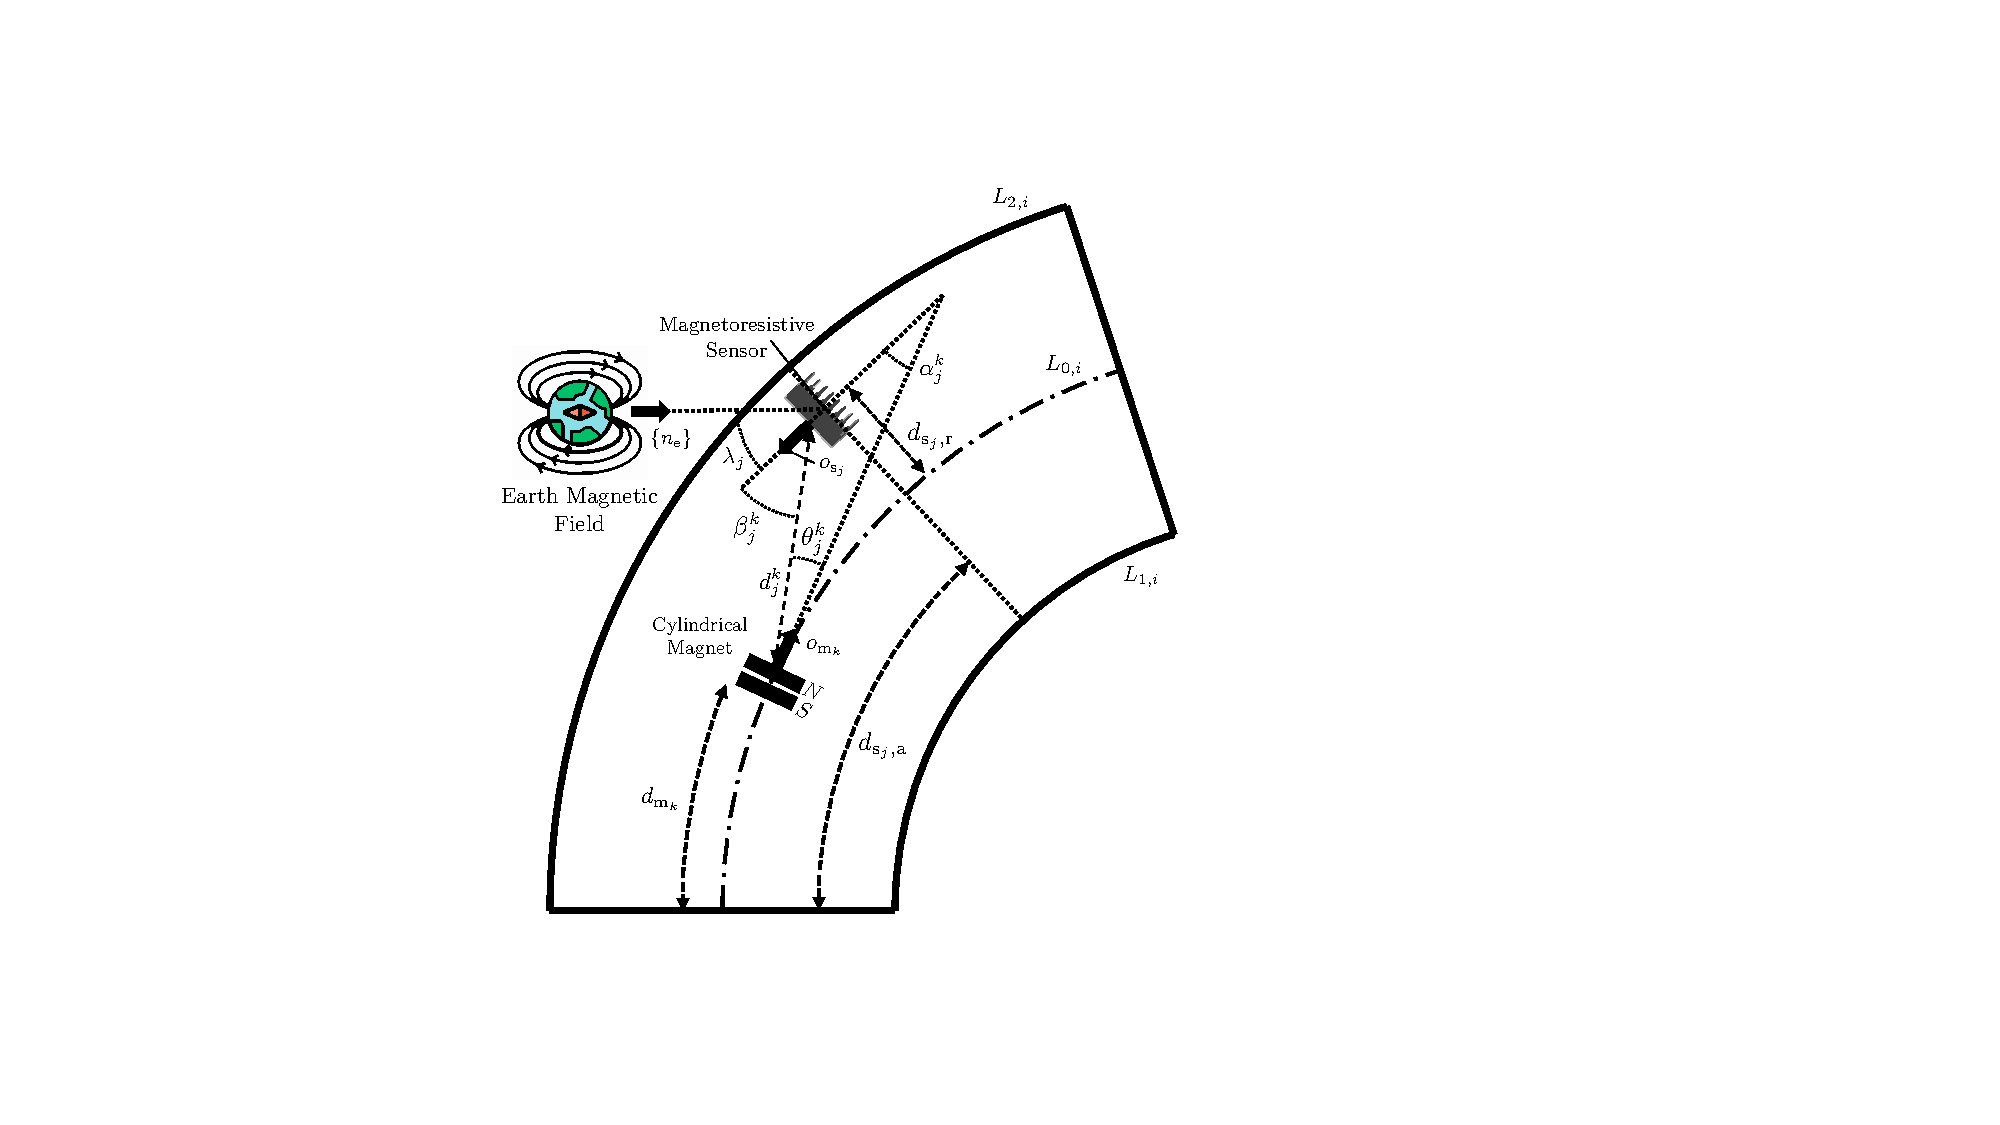
\includegraphics[width=0.5\columnwidth]{promasens/figures/methodology/magnet_sensor_kinematics_v5_compressed.pdf}\label{fig:promasens:magnet_sensor_kinematic}}
\subfigure[Coordinate transformations]{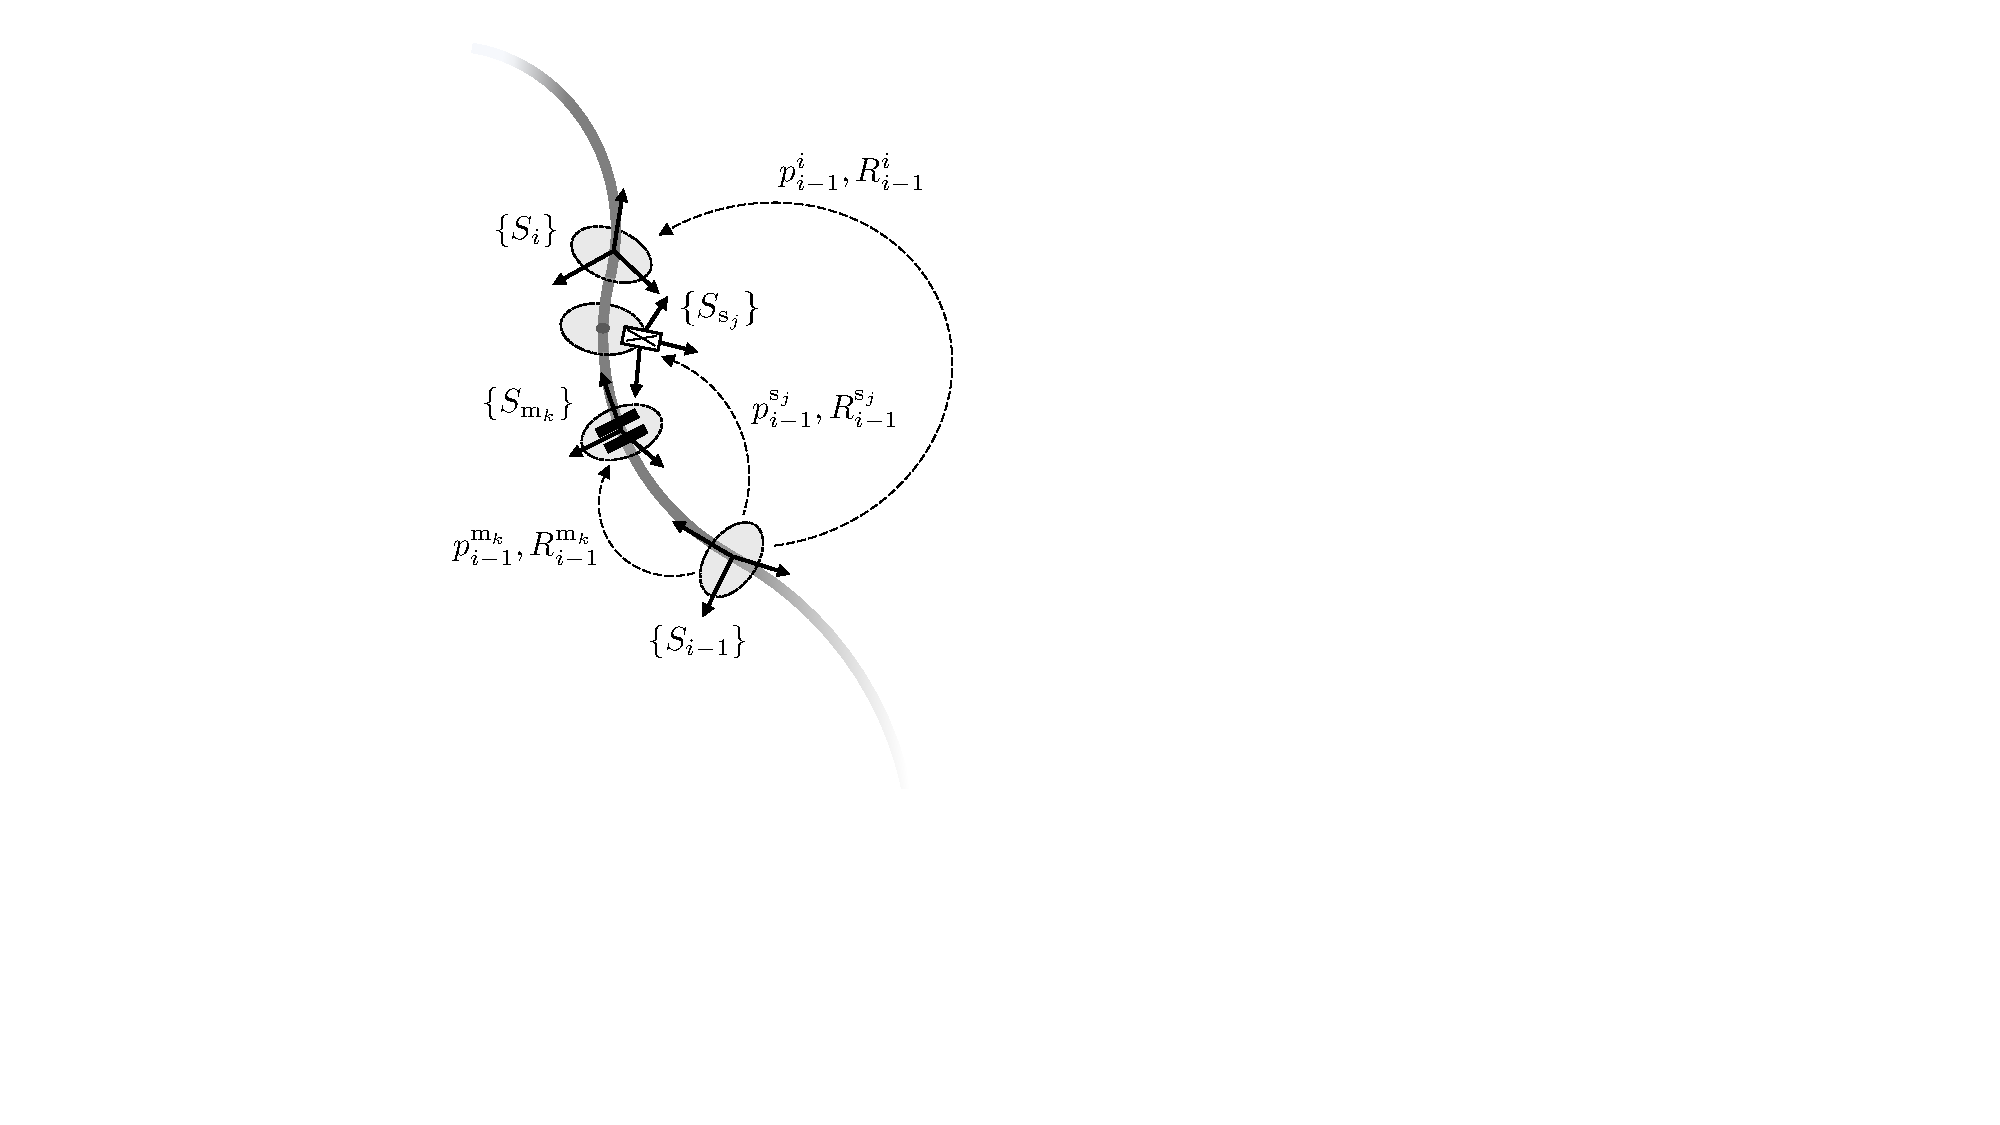
\includegraphics[width=0.4\columnwidth]{promasens/figures/methodology/kinematic_frames_v5_cropped.pdf}\label{fig:promasens:kinematics_frames_soft_segment}}
\caption{\textbf{Panel (a):} Parameters used to describe the kinematics between the $j^\mathrm{th}$ sensor and the $k^\mathrm{th}$ magnet. To simplify the illustration, we visualize the unextended planar case with both magnet and sensor part of the $i^\mathrm{th}$ segment. However, this is not a strict assumption as magnets and sensors can also be part of different segments. \textbf{Panel (b):} Coordinate frames for a soft segment containing the $j^\mathrm{th}$ magnetoresistive sensor and the $k^\mathrm{th}$ cylindrical magnet placed along the center line. $\{S_{i-1}\}$ and $\{S_{i}\}$ describe the frames of the base and tip of the $i^\mathrm{th}$ segment, respectively.}
\end{figure}

\section{Background: Continuum soft robot kinematics}\label{sec:promasens:kinematics}
A kinematic description provides us with the forward kinematic transformation $T_{i-1}^s(q_i,s)$ from base frame $\{S_{i-1}\}$ at the proximal end of the $i^\mathrm{th}$ segment to the local frame $\{S_{v}\}$ at a coordinate $v \in [0,1]$ for a given configuration $q_i$. Furthermore, the tip frame of the $i^\mathrm{th}$ segment located at the coordinate $v = 1$ is denoted as $\{S_{i}\}$, as shown in Fig.~\ref{fig:promasens:kinematics_frames_soft_segment}.

\subsection{Piecewise constant curvature kinematics}\label{sub:promasens:kinematic_model_pcc}

Under the \gls{PCC} hypothesis, the shape of each segment $i$ of length $L_{i}$ and radius $d_i$ can be fully parameterized through three variables
\begin{equation}
    q_i = \begin{bmatrix}\Delta_{x,i} & \Delta_{y,i} & \delta L_{i} \end{bmatrix}^{\mathrm{T}} \in \mathbb{R}^3
\end{equation}
where $\Delta_{x,i}$ and $\Delta_{y,i}$ represent bending into the local $x$ and $y$ directions respectively and $\delta L_i$ defines the elongation of the segment.
The base frame of segment $i$ is referred to as $\{S_{i-1}\}$ as stated in Fig.~\ref{fig:promasens:kinematics_frames_soft_segment}. Given $q_i$, a homogeneous transformation $T_{i-1}^{v}(q_i, v)$ to the point frame $\{S_{v}\}$ is available
\begin{equation}
\label{eq:promasens:transform_improved_q}
\begin{split}
    R_{i-1}^{v}(q_i,v) &=
    \begin{bmatrix}
        1 + \frac{\Delta_{x,i}^2}{\Delta_{i}^2} \left ( \mathrm{C}_v - 1 \right ) & \frac{\Delta_{x,i} \Delta_{y,i}}{\Delta_{i}^2} \left ( \mathrm{C}_v - 1 \right ) & \frac{\Delta_{x,i}}{\Delta_i} \mathrm{S}_v\\
        \frac{\Delta_{x,i} \Delta_{y,i}}{\Delta_{i}^2} \left ( \mathrm{C}_v - 1 \right ) & 1 + \frac{\Delta_{y,i}^2}{\Delta_{i}^2} \left ( \mathrm{C}_v - 1 \right ) & \frac{\Delta_{y,i}}{\Delta_i} \mathrm{S}_v\\
        \frac{-\Delta_{x,i}}{\Delta_i} \mathrm{S}_v & \frac{-\Delta_{y,i}}{\Delta_i} \mathrm{S}_v & \mathrm{C}_v
    \end{bmatrix},\\
    p_{i-1}^{i}(q_i,v) &= \frac{d_i ( L_{0,i}+\delta L_i)}{v \, \Delta_i^2}
    \begin{bmatrix}
        \Delta_{x,i} (1 - \mathrm{C}_v) & \Delta_{y,i} (1 - \mathrm{C}_v) & \Delta_{i} \mathrm{S}_v,
    \end{bmatrix}^{\mathrm{T}}
\end{split}
\end{equation}
where $R_{i-1}^{v}$, $p_{i-1}^{i}(q_i,v)$ denote the rotation matrix and translation vector respectively. We substituted $\Delta_i = \sqrt{\Delta_{x,i}^2 + \Delta_{y,i}^2}$, $\mathrm{S}_v = \sin \left (\frac{v \, \Delta_i}{d_i} \right )$, and $\mathrm{C}_v = \cos \left ( \frac{v \, \Delta_i}{d_i} \right )$ for conciseness.

\subsection{Affine curvature kinematics}\label{sub:promasens:kinematic_model_ac}
The affine curvature hypothesis~\cite{della2020soft, stella2023piecewise} models the bending of the soft segment to be conforming to the affine function $\kappa(t,v) = \kappa_0(t) + \kappa_1(t) v$, where $\kappa$ describes the local curvature of the backbone at the coordinate $v \in [0, 1]$ along the segment and $\kappa_0(t)$, $\kappa_1(t)$ are the zero-order and first-order term of the curvature polynomial respectively~\cite{della2019control}.
Specifically, we implement the recently proposed extension to 3D environments~\cite{stella2023piecewise}, which specifies an azimuth angle of the bending direction $\phi(t)$ and additionally allows for an elongation $\delta L(t)$ of the segment.
% We extend this parametrization as introduced by Della Santina et al.~\cite{della2019control, della2020soft} to 3D environments by specifying the azimuth angle of the bending direction $\phi(t)$ and additionally allowing for an elongation $\delta L(t)$ of the segment. 
Accordingly, the configuration of the $i^\mathrm{th}$ segment is described at any point in time by
\begin{equation}
    q_i = \begin{bmatrix}\kappa_{0,i} & \kappa_{1,i} & \phi_i & \delta L_{i} \end{bmatrix}^{\mathrm{T}} \in \mathbb{R}^4.
\end{equation}
Now that the configuration space is defined, we aim to find a description of the forward kinematics. Firstly, the bending angle $\theta_i(q, v)$ is found by integrating the curvature
\begin{equation}
    \theta(q,v) = \int_{v'=0}^{v} \kappa_i(q, v') \, \mathrm{d}v' = \kappa_{0,i} \, v + \kappa_{1,i} \, \frac{v^2}{2}.
\end{equation}
The rotation to the frame $\{S_{v}\}$ can then be easily determined with $R_{i-1}^{i}(q,v) = R_{\phi_i}(q,v) \, R_{\theta}(q,v) R_{\phi_i}^\mathrm{T}(q,v)$. After substituting $S_{\cdot} = \sin(\cdot)$, $C_{\cdot} = \cos(\cdot)$ for conciseness, we state the homogeneous transformation as
\begin{equation}\label{eq:promasens:affine_curvature_forward_kinematics}
\begin{split}
    R_{i-1}^v(q,v) &= \begin{bmatrix}
        S_{\phi_i}^2 C_{\theta_v} + C_{\phi_i}^2 & -S_{\phi_i} C_{\phi_i} C_{\theta_i} + S_{\phi_i}C_{\phi_i} & S_{\phi_i} S_{\theta_v}\\
        -S_{\phi_i} C_{\phi_i} C_{\theta_i} + S_{\phi_i} C_{\phi_i} & S_{\phi_i}^2 + C_{\phi_i}^2 C_{\theta_v} & -S_{\theta_v} C_{\phi_i}\\
        -S_{\phi_i} S_{\theta_v} & S_{\theta_v} C_{\phi_i} & C_{\theta_i}
    \end{bmatrix},\\
    p_{i-1}^{v}(q,v) &= \left ( L_{0,i} + \delta L_i \right ) \, \begin{pmatrix}
        \int_{v'=0}^{v} \sin(\theta(q, v')) \, \mathrm{d}v' \, \sin(\phi_i)\\
        - \int_{v'=0}^{v} \sin(\theta(q, v')) \, \mathrm{d}v' \, \cos(\phi_i)\\
        \int_{v'=0}^{v} \cos(\theta(q, v')) \, \mathrm{d}v'
    \end{pmatrix}.
\end{split}
\end{equation}
We choose to integrate the translational terms in \eqref{eq:promasens:affine_curvature_forward_kinematics} numerically with $101$ sample points using the Torchquad~\cite{gomez2021torchquad} implementation of the Simpson's rule, which makes the forward kinematics fully and automatically differentiable.


\subsection{Magnet sensor kinematics}\label{sub:promasens:kinematic_model_magnet_sensor_kinematics}
This subsection derives the kinematic relationship $\xi_j = f_{\xi_j}(q) \in \mathbb{R}^{1+4n_\mathrm{m}}$ between the $j^\mathrm{th}$ sensor and all $n_\mathrm{m}$ magnets as we hypothesize that we can estimate the sensor measurement $u_j$ solely based on
a) the angle $\lambda_j \in \mathbb{R}^1$ to the earth's magnetic field,
b) the distance $d_j^k$  between the $j^\mathrm{th}$ sensor and $k^\mathrm{th}$ magnet,
c) the angle $\alpha_j^k$ between the sensor measurement direction and the cylindrical axis of the magnet,
d) the angle $\beta_j^k$ between the sensor measurement direction and the vector from the magnet to the sensor,
and e) the angle $\theta_j^k$ between the cylindrical axis of the magnet and the vector from the magnet to the sensor.
Accordingly, $\xi_j$ is defined as
\begin{equation}
    \xi_{j} = f_{\mathrm{\xi},j}(q) =
    \begin{pmatrix}
        \lambda_{j} & {\xi_{j}^1}^\mathrm{T} & \cdots & {\xi_{j}^k}^\mathrm{T} & \cdots & {\xi_{j}^{n_\mathrm{m}}}^\mathrm{T}
    \end{pmatrix}^\mathrm{T} \in \mathbb{R}^{1 + 4n_\mathrm{m}},
\end{equation}
with $\xi_j^{k} \in \mathbb{R}^4$ the kinematic relationship between the $j^\mathrm{th}$ sensor and the $k^\mathrm{th}$ magnet: $\xi_j^{k} = \begin{pmatrix} d_j^k & \alpha_j^k & \beta_j^k & \theta_j^k \end{pmatrix}^\mathrm{T} \in \mathbb{R}^4$. We visualize the parameters incorporated in $\xi_j^{k}$ in Fig.~\ref{fig:promasens:magnet_sensor_kinematic}.
% \begin{equation}
%     \xi_j^{k} = \begin{pmatrix} d_j^k & \alpha_j^k & \beta_j^k & \theta_j^k \end{pmatrix}^\mathrm{T}.
% \end{equation}

In the following, we present the derivation of all components of $\xi_j^{k}$. 
Please note that all kinematic frames used in the following paragraphs are visualized in Fig.~\ref{fig:promasens:kinematics_frames_soft_segment}.
% \textcolor{blue}{All the kinematic frames introduced over the last few paragraphs are visualized in Fig.~\ref{fig:promasens:kinematics_frames_soft_segment}}.

We define that the $k^\mathrm{th}$ magnet is integrated into the $i^\mathrm{th}$ segment. Now, we first derive a transformation matrix $T_{i-1}^{\mathrm{m}_k}$ from the base frame $\{S_{i-1}\}$ to the magnet frame $\{ S_{\mathrm{m}_k} \}$. 
This can be achieved by evaluating the chosen kinematic model, two of which we report in the Appendix~\ref{sec:promasens:kinematics}, at the segment coordinate $v = \frac{d_{\mathrm{m}_k}}{L_{0,i}}$. 
This means that the cylindrical magnet is integrated at a distance, which is measured along the backbone, of $d_{\mathrm{m}_k}$ from the base of the segment.
% The cylindrical magnet is integrated into the segment at an axial distance of $d_{\mathrm{m}_k}$ from $\{S_{i-1}\}$.
% We compute the translational and rotational components of the transformation matrix $p_{i-1}^{\mathrm{m}_k}$ and $R_{i-1}^{\mathrm{m}_k}$ \textcolor{blue}{by evaluating the forward kinematics $T_{i-1}^v(q_i,v)$, which are reported in Appendix~\ref{sec:promasens:kinematics}, at the point $v = \frac{d_{\mathrm{m}_k}}{L_{0,i}}$.}

% as in \cite{della2020improved} by substituting $\Delta_{x}^{\mathrm{m}_k} = \frac{d_{\mathrm{m}_k}}{L_{0,i}} \, \Delta_{x,i}$, $\Delta_{y}^{\mathrm{m}_k} = \frac{d_{\mathrm{m}_k}}{L_{0,i}} \, \Delta_{y,i}$ and $\Delta_{\mathrm{m}_k} = \frac{d_{\mathrm{m}_k}}{L_{0,i}} \, \Delta_{i}$. % in \eqref{eq:promasens:transform_improved_q}.

Subsequently, we  describe the pose of the $j^\mathrm{th}$ sensor with respect to the base of the $i^\mathrm{th}$ segment.
Denote with $d_{\mathrm{s}_j,\mathrm{r}}$ the radial distance of the sensor from the center line, with $\varphi_j$ the azimuth angle of the sensor in the cylindrical plane, and with $d_{\mathrm{s}_j,\mathrm{a}}$ the axial distance along the center line from the base of the $i^\mathrm{th}$ segment.
We derive the transformation $T_{i-1}^{\mathrm{s}_j,\mathrm{r}_0}$ to the center of the cylindrical plane of the sensor % using \eqref{eq:promasens:transform_improved_q}
analogously as for the magnets by evaluating the forward kinematics at $v = \frac{d_{\mathrm{s}_j,\mathrm{a}}}{L_{0,i}}$.
% by scaling the configuration vector $q_i$ with $\frac{d_{\mathrm{s}_j,\mathrm{a}}}{L_{0,i}}$ in the transformation matrix~\cite{della2020improved}.
This is followed by applying the radial offset $d_{\mathrm{s}_j,\mathrm{r}}$ in the cylindrical plane of the sensor
% \begin{equation}
% \begin{split}
%     t_{i-1}^{\mathrm{s}_j} = t_{i-1}^{\mathrm{s}_j,\mathrm{r}_0} + R_{i-1}^{\mathrm{s}_j,\mathrm{r}_0} \, d_{\mathrm{s}_j,\mathrm{r}}
%     \,
%     \begin{pmatrix}
%         \cos{\varphi_j} & \sin{\varphi_j} & 0
%     \end{pmatrix}^{\mathrm{T}}.
% \end{split}
% \end{equation}
\begin{equation}
    T_{i-1}^{\mathrm{s}_j} = T_{i-1}^{\mathrm{s}_j,\mathrm{r}_0}
    \,
    \begin{bmatrix}
        \cos{\varphi_j} & - \sin{\varphi_j} & 0 & d_{\mathrm{s}_j} \cos(\varphi_j)\\
        \sin{\varphi_j} & \cos{\varphi_j} & 0 & d_{\mathrm{s}_j} \sin(\varphi_j)\\
        0 & 0 & 1 & 0\\
        0 & 0 & 0 & 1\\
    \end{bmatrix}.
\end{equation}
Optionally, a static rotation offset can be applied to $R_{i-1}^{\mathrm{s}_j}$ such that local z-axis $\{ o_{\mathrm{s}_j} \}$ corresponds to the sensor measurement direction.
% Hereafter, we will assume that the measurement direction of the sensor points along the local positive  z-axis and any other orientation is compensated by adding a static rotation offset to $R_{i-1}^{\mathrm{s}_j}$.

Knowing the transformation matrices from the base frame of the respective segment to the sensor and magnet frames, we express them in the inertial frame $\{S_{0}\}$ by multiplying with the kinematic chain $T_{0}^{i-1} = \Pi_{\bar{i}=1}^{i-1} \, T_{\bar{i}-1}^{\bar{i}}$.

Next, we need to express the sensor measurement direction $\{ o_{\mathrm{s}_j} \}_{0}$ and the cylindrical axis of the magnet $\{ o_{\mathrm{m}_k} \}_{0}$ in the inertial frame
\begin{equation}
    \{ o_{\mathrm{s}_j} \}_{0} = R_{0}^{\mathrm{s}_j}
    \begin{pmatrix}
        0 & 0 & 1
    \end{pmatrix}^{\mathrm{T}},
    \quad
    \{ o_{\mathrm{m}_k} \}_{0} = R_{0}^{\mathrm{m}_k}
    \begin{pmatrix}
        0 & 0 & 1
    \end{pmatrix}^{\mathrm{T}}.
\end{equation}
% and analogue for the cylindrical axis of the magnet $\{ \hat{o}_{\mathrm{m}_k} \}_{0}$
% \begin{equation}
%     \{ \hat{o}_{\mathrm{m}_k} \}_{0} = R_{0}^{\mathrm{m}_k}
%     \begin{pmatrix}
%         0 & 0 & 1
%     \end{pmatrix}^{\mathrm{T}}.
% \end{equation}
%
As the sensor measures contributions of the earth's magnetic field, we need to state the angle $\lambda_{j}$ between $\{ o_{\mathrm{s}_j} \}_0$ and the earth's magnetic field unit vector $\{ n_{\mathrm{e}} \}_{0}$. 
Similarly, we investigate the angle $\alpha_j^k$ between $\{ o_{\mathrm{s}_j} \}_{0}$ and the cylindrical axis of the magnet $\{ o_{\mathrm{m}_k} \}_{0}$
\begin{equation}
    \cos (\lambda_{j}) = \{n_{\mathrm{e}} \}_{0} \cdot \{ o_{\mathrm{s}_j} \}_{0},
    \quad
    \cos (\alpha_{j}^k) = \{ o_{\mathrm{m}_k} \}_{0} \, \{ o_{\mathrm{s}_j} \}_{0}.
\end{equation}
% While $\{ \hat{n}_{\mathrm{e}} \}_{0}$ is dependent on the exact experimental setup, we report for the special case of the z-axis of the $\{S_{0}\}$ frame being perpendicular to the earth surface with a compass displaying an angle of $\varphi_e$ to the x-axis the following relation
% \begin{equation}
%     \{ \hat{n}_{\mathrm{e}} \}_{0} =
%     \begin{pmatrix}
%         \cos(\varphi_e) & \sin(\varphi_e) & 0
%     \end{pmatrix}^{\mathrm{T}}.
% \end{equation}
% Next, we investigate the angle $\alpha_j^k$ between the sensor measurement direction $\{ \hat{o}_{\mathrm{s}_j} \}_{0}$ and the cylindrical axis of the magnet $\{ \hat{o}_{\mathrm{m}_k} \}_{0}$
% \begin{equation}
%     \cos (\alpha_{j}^k) = \{ \hat{o}_{\mathrm{m}_k} \}_{0} \, \{ \hat{o}_{\mathrm{s}_j} \}_{0}.
% \end{equation}
We define the translation and distance between the magnet and the sensor in the frame $\{S_{0}\}$ as:
\begin{equation}\label{eq:promasens:t_jk_and_d_jk}
    p_j^{k} = p_{0}^{\mathrm{s}_j} - p_{0}^{\mathrm{m}_k}, \qquad  d_j^k = \lVert p_{j}^{k} \rVert_2.
\end{equation}
% This lets us find the distance between the sensor and the magnet with the Euclidean norm
% \begin{equation}\label{eq:promasens:d_jk}
%     d_j^k = \lVert t_{j}^{k} \rVert_2.
% \end{equation}
Building on the derivation in \eqref{eq:promasens:t_jk_and_d_jk}, we compute the angles $\beta_j^k$ and $\theta_j^k$ using the dot product rule
\begin{equation}\label{eq:promasens:theta_jk_and_beta_jk}
    \cos (\beta_j^k) = \frac{p_j^{k} \, \{ o_{\mathrm{s}_j} \}_{0}}{\lVert p_j^{k} \rVert}_2,
    \qquad
    \cos (\theta_j^k) = \frac{p_j^{k} \, \{ o_{\mathrm{m}_k} \}_{0}}{\lVert p_j^{k} \rVert}_2.
\end{equation}
Lastly, the kinematic descriptions for all sensors are vertically stacked as
\begin{equation}
    \xi = \begin{pmatrix} \xi_1^\mathrm{T} \dots \xi_j^\mathrm{T} \dots \xi_{n_\mathrm{s}}^\mathrm{T} \end{pmatrix}^\mathrm{T} \in \mathbb{R}^{n_\mathrm{s} + 4n_\mathrm{m} n_\mathrm{s}}.
\end{equation}
% $\xi_j(t) \in \mathbb{R}^{1 + 4n_\mathrm{m}}$
% $\xi(t) = f_\xi(q(t)) \in \mathbb{R}^{n_\mathrm{s} + 4n_\mathrm{m} n_\mathrm{s}}$
We will in the following refer to the mapping $f_\xi(q): q \in \mathbb{R}^{n_\mathrm{q}}
\rightarrow \xi \in \mathbb{R}^{n_\mathrm{s} + 4n_\mathrm{m} n_\mathrm{s}}$ as the magnet sensor kinematics.


\begin{algorithm}[hbt!]
\caption{Proprioception with magnetic sensors}\label{alg:proprioception}
\begin{algorithmic}
\REQUIRE $u(t) \in \mathbb{R}^{n_\mathrm{s}}$ \COMMENT{Sensor measurements}
\STATE  \hspace{7mm} $\hat{q}(t-1) \in \mathbb{R}^{3n_\mathrm{b}}$
\COMMENT{Configuration of prev. time-step}
\STATE  \hspace{7mm} $\hat{q}_\mathrm{glob}^*(t-\delta) \in \mathbb{R}^{3n_\mathrm{b}}$
\COMMENT{Solution of grid search $\delta$ ago}
\STATE  \hspace{7mm} $f_\xi: \mathbb{R}^{2n_\mathrm{b}} \rightarrow \mathbb{R}^{n_\mathrm{s} + 4n_\mathrm{m} n_\mathrm{s}}$ \COMMENT{Magnet Sensor Kin.}
\STATE  \hspace{7mm} $f_\pi: \mathbb{R}^{n_\mathrm{s} + 4n_\mathrm{m} n_\mathrm{s}} \rightarrow \mathbb{R}^{n_\mathrm{s}}$ \COMMENT{Trained neural network}
\ENSURE $\hat{q}(t) \in \mathbb{R}^{2n_\mathrm{b}}$ \COMMENT{Estimated robot configuration}
    \IF{gridSearchIsFinished()}
        \STATE $\hat{q}_0 \gets \hat{q}_\mathrm{glob}^*(t-\delta)$
    \ELSE
        \STATE $\hat{q}_0 \gets \hat{q}(t-1)$
    \ENDIF
    \vspace{0.25em}
    \STATE $l \gets 0$
    \STATE $b_l \gets 0 \in \mathbb{R}^{3n_\mathrm{b}}$
    \vspace{0.25em}
    % \WHILE{$\left|\Omega \right| >\epsilon$}
    \WHILE{$l < n_\mathrm{it}$}
    \vspace{0.25em}
    \STATE $\hat{\xi}_l \gets f_{\xi}(\hat{q}_{l})$
    \vspace{0.25em}
    \STATE $\hat{u}_l \gets f_\pi(\hat{\xi}_l)$
    \vspace{0.25em}
    \STATE $\hat u_{l}^{\mathrm{error}} \gets \lVert \hat{u}_{l}-u(t) \rVert_2$
    \vspace{0.25em}
    % \STATE $\frac{\partial}{\partial \hat{q}_l} \mathcal{L}_{u}(\hat{q}_l) \gets \frac{2}{n_\mathrm{s}} \frac{\partial }{\partial {\hat{q}_l}} f_{\mathrm{\xi}}^\mathrm{T}(\hat{q}_l) \, \frac{\partial}{\partial {\hat{\xi}_l}} f_\pi^\mathrm{T}(\hat{\xi}_l) \, (\hat{u}_l - u(t))$
    \STATE $b_{l+1} \gets \mu \, b_l + \frac{2}{n_\mathrm{s}} \frac{\partial }{\partial {\hat{q}_l}} f_{\mathrm{\xi}}^\mathrm{T}(\hat{q}_l) \, \frac{\partial}{\partial {\hat{\xi}_l}} f_\pi^\mathrm{T}(\hat{\xi}_l) \, (\hat{u}_l - u(t))$
    % \vspace{0.25em}
    \STATE $\hat{q}_{l+1} \gets \hat{q}_l - \gamma \, b_{l+1} $
    % \vspace{0.25em}
    % \textcolor{orange}{\STATE $ \Omega \gets \mathrm{RMSE}(\hat{u}_{l+1}^{error})-\mathrm{RMSE}(\hat{u}_{l-n_\mathrm{p}}^{error})$ \COMMENT{Early Stopping Criteria with patience $n_\mathrm{p}$}}
    \vspace{0.25em}
    \STATE $l \gets l + 1$
\ENDWHILE
\STATE $l^* \gets \mathrm{argmin}_{l} \, u_{l}^{error}$
\STATE $\hat{q}(t) \gets \hat{q}_l^{*}$
\end{algorithmic}
\end{algorithm}

\begin{figure}[ht]
\centering
    % \subfigure[Optimization scheduling]{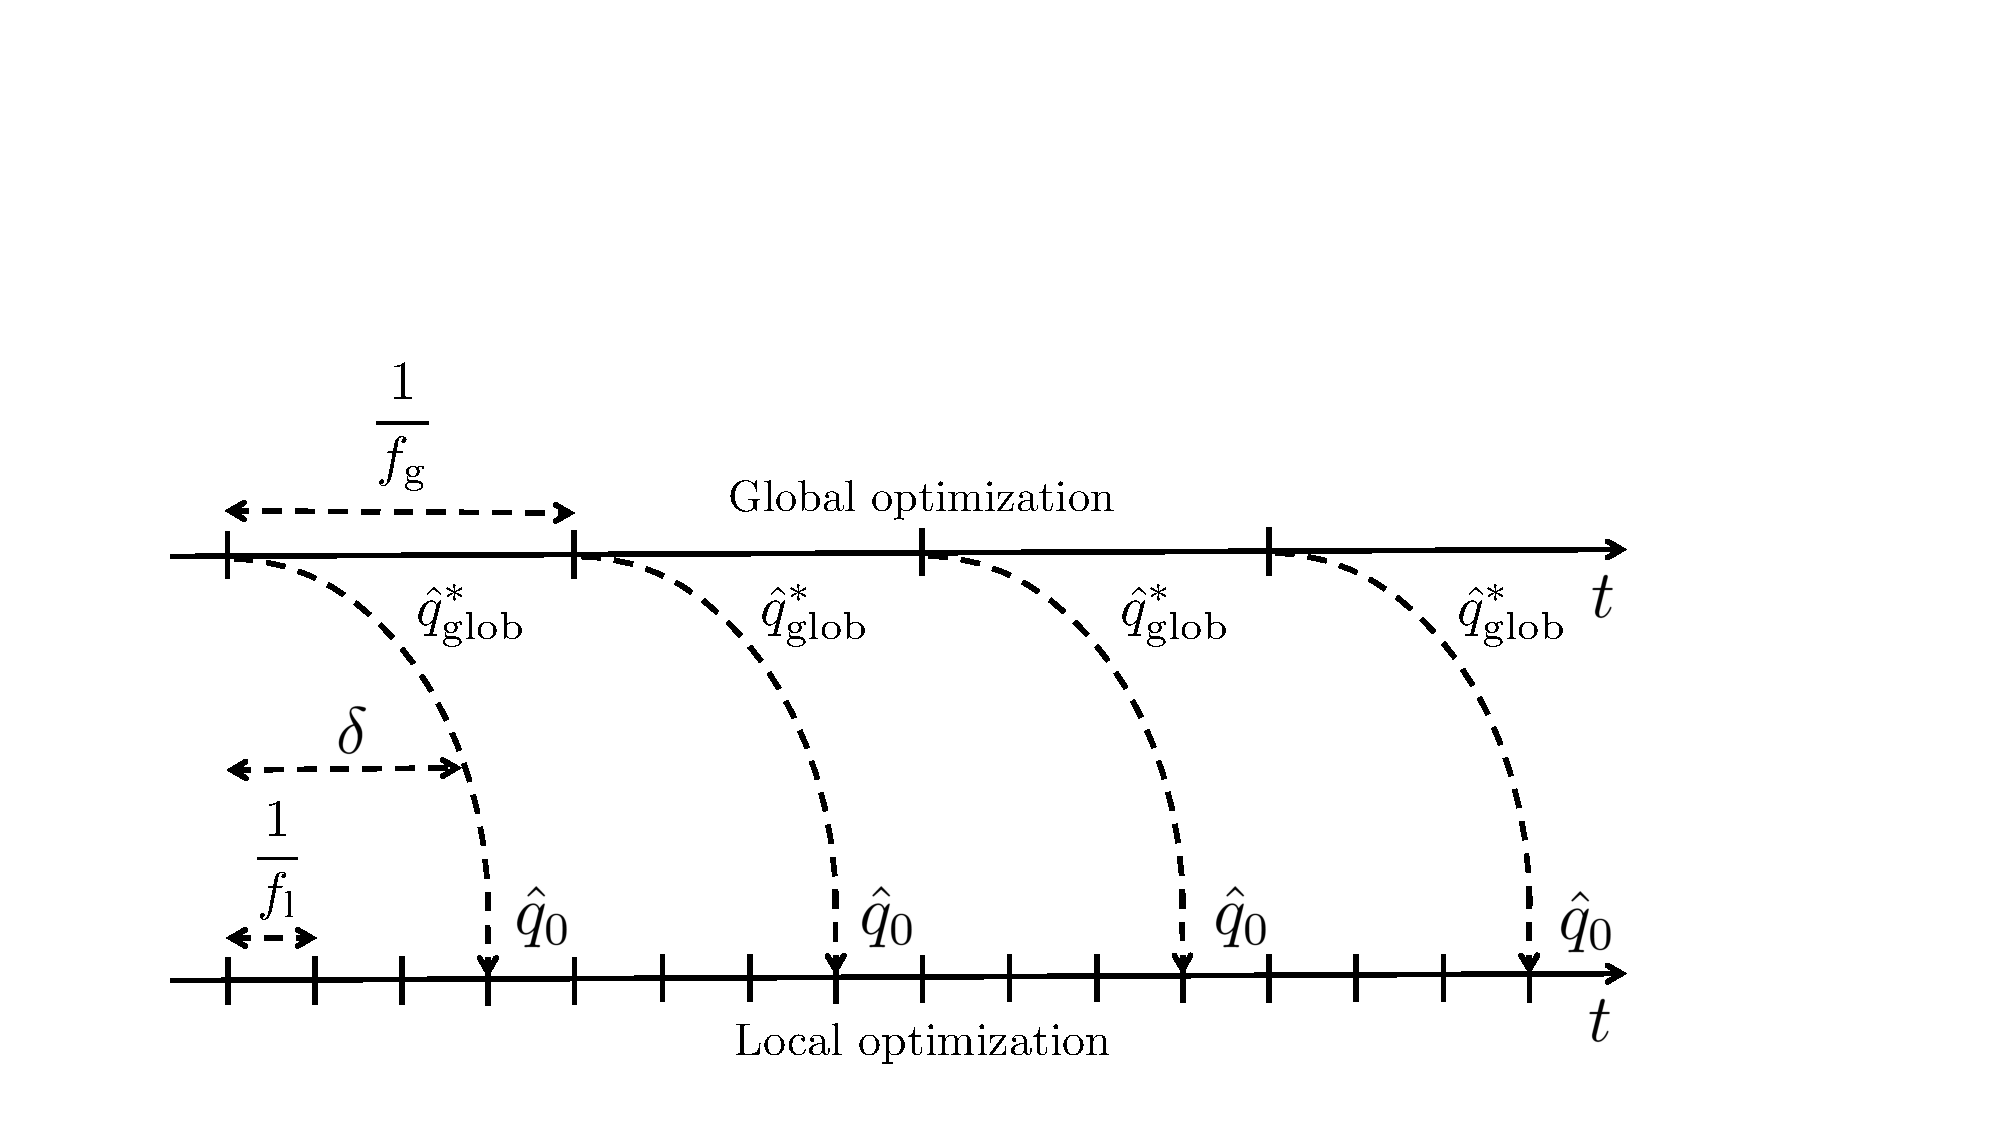
\includegraphics[width=1.0\columnwidth]{promasens/figures/methodology/optimization_scheduling_v2_cropped.pdf}\label{fig:promasens:optimization_scheduling}}\\
    % \subfigure[Local optimization: gradient descent]{\includegraphics[width=1.0\columnwidth]{promasens/figures/methodology/blockdiagram_gradient_descent_v4_cropped.pdf}\label{fig:promasens:blockdiagram_gradient_descent}}
    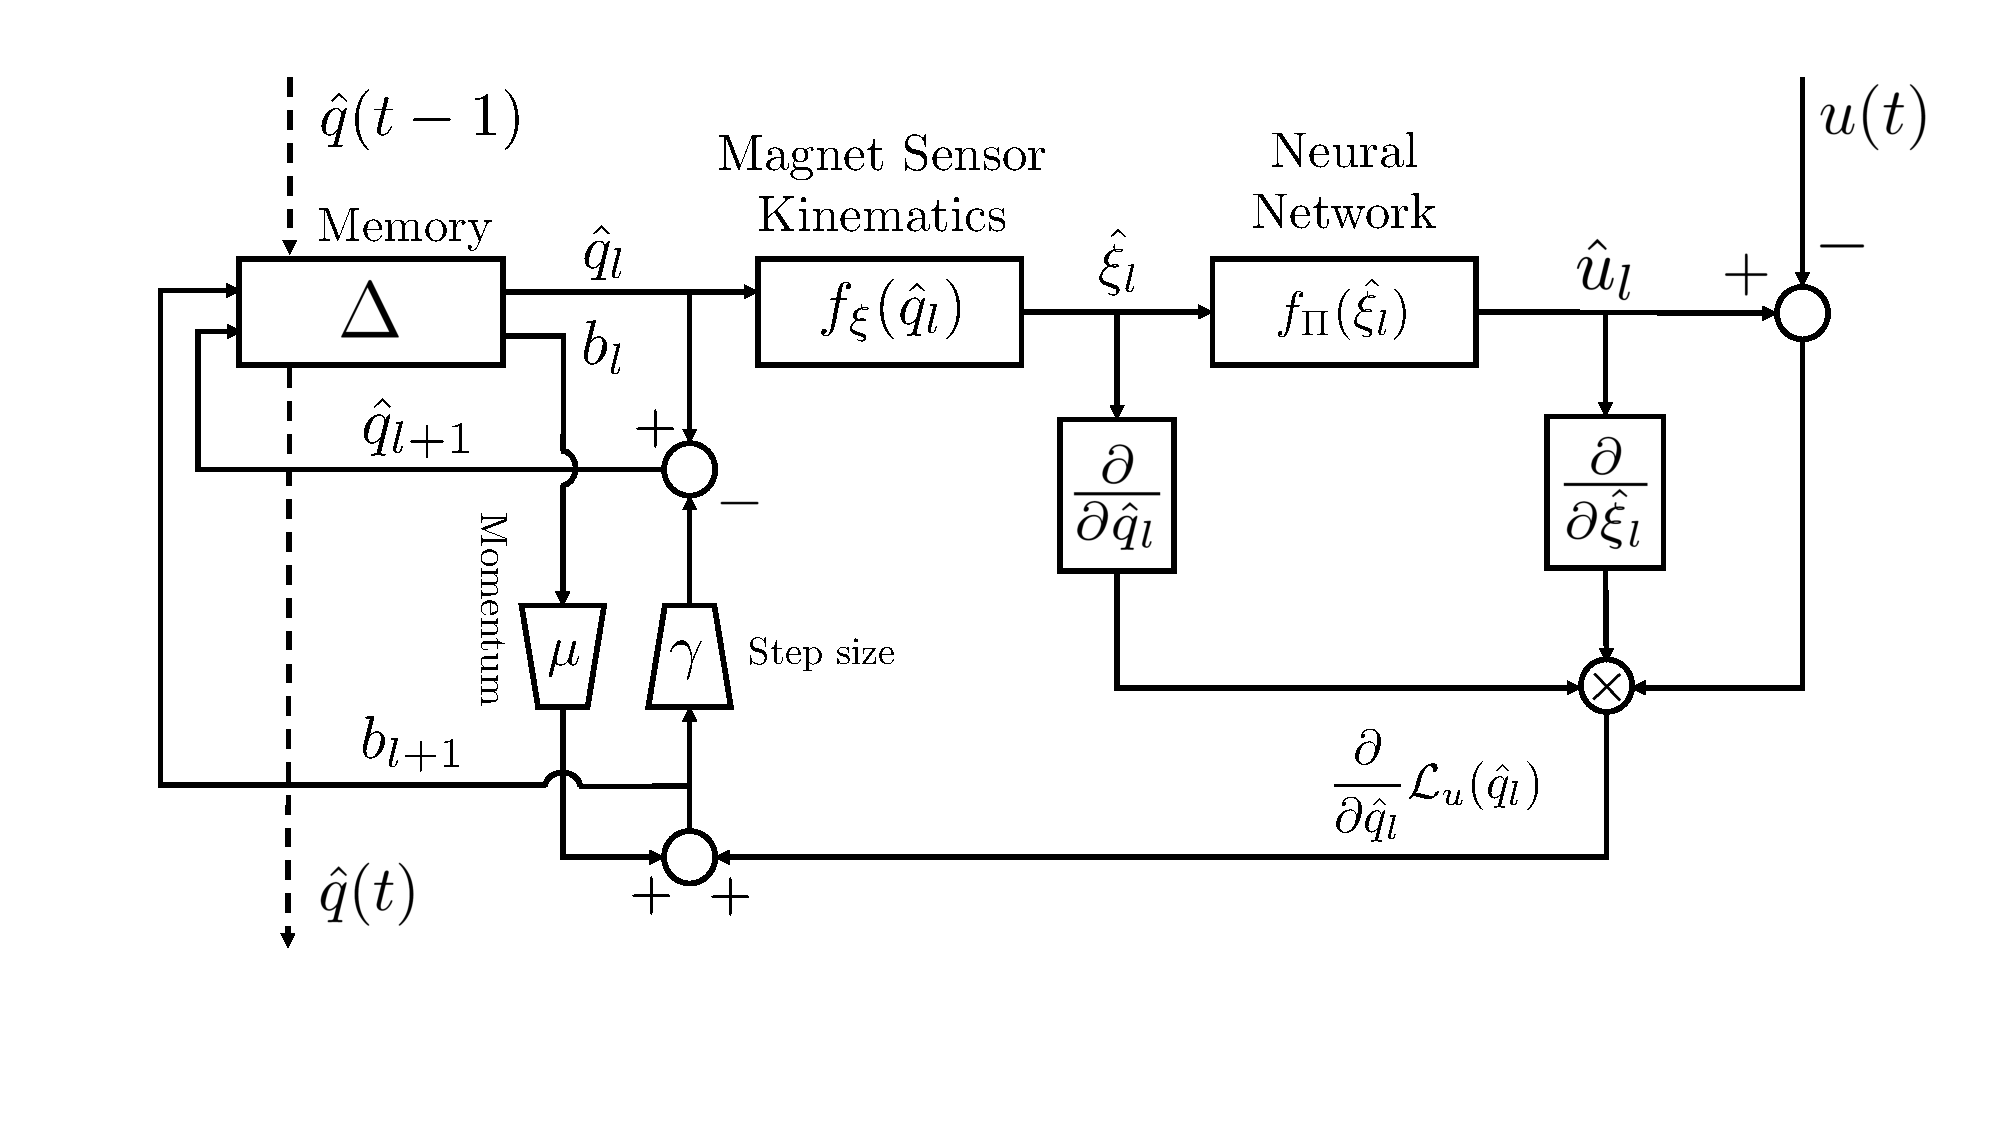
\includegraphics[width=0.8\columnwidth]{promasens/figures/methodology/blockdiagram_gradient_descent_v6_cropped.pdf}
    \caption{% In panel (a), we visualize the scheduling of our chosen optimization strategy: global optimization involving grid search is running at a frequency $f_\mathrm{g}$. In parallel, local gradient descent is performed at a frequency $f_\mathrm{l}$. The global optimization solution arrives $\hat{q}_\mathrm{glob}^*(t-\delta)$ at the local optimization with a delay of $\delta$ and is used to initialize $\hat{q}_0$ for the gradient descent. In all other instances, the gradient descent is initialized with the locally optimized solution $\hat{q}(t-1)$ from the previous time-step. 
    % Panel (b) 
    A block-diagram of the gradient descent as an iterative update loop for the configuration belief $\hat{q}(t)$. The gradient descent is initialized with the optimized solution $\hat{q}_0 = \hat{q}(t-1)$ from the previous time-step. Note that during the iterative loop, $\hat{q}_{l+1}$ updates $\hat{q}_{l}$ in the memory block.}\label{fig:promasens:blockdiagram_gradient_descent}
\end{figure}


\subsection{Data-driven sensor measurement model}
\label{sec:promasens:data_driven_approach}
We use a data-driven approach to learn the forward sensor model $\hat{u} = f_{\pi}(\xi_{j})$ for each sensor using a neural network parameterized with $\pi$.
We note that the same neural network weights can be shared for all sensors, but oftentimes performance can be improved by training a specialized model with weights $\pi_j$ for each sensor.
During training on a dataset of length $n_\mathrm{t}$, we minimize the Mean Squared Error (MSE) error between the predicted sensor measurement $\hat{u}_j$ and the actual sensor measurement $u_j$:
\begin{equation}
    \min_{\pi} \frac{1}{n_\mathrm{t}} \sum_{t = 0}^{n_\mathrm{t}} \left ( f_{\pi}(\xi_{j}(t)) - u_j(t) \right )^2,
\end{equation}
where $t$ denotes the current time index.
Note that whenever we omit the time index in our notation, we always refer to the current time $t$.
Finally, to simplify the notation, we combine each sensor measurement prediction $u_j \in \mathbb{R}$ into an array $u \in \mathbb{R}^{n_\mathrm{s}}$ and stack the neural networks as %$u = f_\pi(\xi)$
$f_\Pi(\xi): \xi \rightarrow u$. We discuss the choice of the specific network architecture later in Section~\ref{sec:promasens:pcc_simulations}.

\subsection{Proprioception by optimizing configuration estimate}
\label{sub:promasens:proprioception_optimization}

Now, that we are able to predict the sensor measurement $\hat{u}$ using the composition of the kinematics $f_\xi(\hat{q})$ and the neural networks $f_\Pi(\hat{\xi})$, we need to optimize the configuration estimate $\hat{q}$ for the predictions $\hat{u}$ to match the actual sensor measurements $u$ as closely as possible.
We capture the error between the predicted sensor measurements $\hat{u}$ and the actual sensor measurements $u$ by the MSE loss function we strive to minimize
\begin{equation}\label{eq:promasens:proprioception_loss}
    \mathcal{L}_{u}(\hat{q}) = \sum_{j=1}^{n_\mathrm{s}} \frac{\left ( f_\pi(\xi_j) - u_j \right )^2}{n_\mathrm{s}}
\end{equation}
Accordingly, the optimal configuration estimate $\hat{q}$ can be found with
\begin{equation}
    \hat{q} = \mathrm{argmin} \: \mathcal{L}_{u}(\hat{q}_l).
\end{equation}

% We employ a dual optimization strategy with global grid search and local gradient descent optimization running in parallel, as visualized in Fig.~\ref{fig:promasens:optimization_scheduling}. As the grid search is computationally expensive, we run it at a frequency of $f_\mathrm{g} \ll f_\mathrm{l}$, where $f_\mathrm{l}$ represents the sampling rate of the gradient descent.
% As we detail in Algorithm~\ref{alg:proprioception}, the gradient descent is nominally initialized with the best estimate of the previous time-step $\hat{q}_0 (t) = \hat{q}(t-1)$.
% When global optimization estimates are available, which are expected to arrive with a computational delay of $\delta$, we use those as an initial condition for the gradient descent.

We optimize the cost function \eqref{eq:promasens:proprioception_loss} through iterative gradient descent, as detailed in Fig.~\ref{fig:promasens:blockdiagram_gradient_descent}. The gradient descent is initialized with the best estimate of the previous time-step $\hat{q}_0 (t) = \hat{q}(t-1)$.
% For the gradient descent itself, detailed in Fig.\ref{fig:promasens:blockdiagram_gradient_descent}, we iteratively
As common in literature, we optimize the state belief $\hat{q}_l$ with a step size $\gamma$ and the momentum $\mu$ using the Jacobian of the loss $\frac{\partial}{\partial \hat{q}_t} \mathcal{L}_{u}(\hat{q})$
\begin{equation}\label{eq:promasens:gradient_descent}
    b_{l+1} = \mu \, b_l + \frac{\partial}{\partial \hat{q}_t} \mathcal{L}_{u}(\hat{q}), \quad \hat{q}_{l+1} = \hat{q}_l - \gamma \, b_{l+1}.
\end{equation}
We can use the chain rule to derive an analytical expression for the gradient of the loss incorporating the gradient of the magnet sensor kinematics $\partial_{\hat{q}} f_{\mathrm{\xi}}(\hat{q})$ and the gradient of the neural network $\partial_{\hat{\xi}} f_\Pi (\hat{\xi})$:
\begin{equation}
    \frac{\partial}{\partial \hat{q}} \mathcal{L}_{u}(\hat{q}) = \frac{2}{n_\mathrm{s}} \left ( \frac{\partial }{\partial {\hat{q}}} f_{\mathrm{\xi}}(\hat{q}) \right )^\mathrm{T} \, \left ( \frac{\partial}{\partial {\hat{\xi}}} f_\Pi(\hat{\xi}) \right )^\mathrm{T} \, (\hat{u} - u).
\end{equation}
After executing the gradient descent for $n_\mathrm{it}$ iterations, we evaluate which iteration $l^*$ had the lowest loss $\mathcal{L}_{u}$ and accordingly select $\hat{q}(t) = \hat{q}_{l^*}$ as the best configuration estimate of time-step $t$.
